
\chapter{نتایج تجربی}

\section{بررسی توابع پیاده‌سازی شده}
در این بخش به بررسی کد موجود برای الگوریتم 
\lr{ISM}
که توسط نویسندگان ارائه شده است می‌پردازیم.
\begin{itemize}
	
\item
\textbf{	تابع 
	\lr{\texttt{./sdr.py}}}

این تابع، مربوط به اجرای تنظیمات اولیه است. با فراخوانی این تابع، دیتاست مورد نظر در 
\lr{db}
قرار گرفته و توسط تمام توابع دیگر قابل دسترسی می‌شود. آستانه‌ی مورد نظر برای پایان الگوریتم ($\delta$) نیز در این تابع تنظیم می‌شود.


\item 
\textbf{	تابع 
\lr{\texttt{./optimizer/ism.py}}}
	
این تابع، پیاده‌سازی الگوریتم 
\lr{ISM}
است. این تابع، ماتریس
$\Phi_0$
را عنوان ورودی دریافت کرده و ماتریس
$\Phi$
 نهایی را باز می‌گرداند.
		 
\item 
\textbf{	توابع فولدر 
\lr{\texttt{./kernels/}}}


در این فولدر، برای هر کرنل یک فایل وجود دارد که در هر فایل، تابعی برای محاسبه‌ی 
$\Phi_0$
و تابعی برای محاسبه‌ی 
$\Phi$
هر کرنل در آن قرار گرفته است.
		
\end{itemize}



\section{نتایج تجربی}
\subsection{توضیح اجمالی در مورد داده‌ها}
در مجموعه داده‌ی 
\lr{Wine}
ویژگی‌ها پیوسته هستند در حالی که در مجموعه‌ی داده‌های 
\lr{Cancer}،
داده‌ها گسسته می‌باشند.  مجموعه‌ی داده‌های
\lr{MNIST}
نیز شامل تصاویری از اعداد انگلیسی به صورت دست‌نوشته است.
\subsection{شرح آزمایش‌ها}

\subsubsection{کاهش بعد نظارت‌شده}
در این آزمایش، ابتدا کاهش بعد انجام می‌شود و سپس بر روی داده‌های کاهش بعد یافته، یک 
\lr{SVM}
آموزش داده‌شده و درصد صحت در 
\lr{10-fold cross validation}
گزارش می‌شود. در هر
\lr{fold}،
ماتریس 
$W$
به کمک الگوریتم 
\lr{ISM}
و تنها با استفاده از داده‌های یادگیری در آن 
\lr{fold}
انجام می‌شود.
\subsubsection{کاهش‌بعد نظارت‌نشده}
بعد از یادگیری
$W$،
بر روی داده‌های کاهش‌بعد یافته، یعنی 
$XW$،
الگوریتم 
\lr{Spectral Clustering}
را اجرا می‌کنیم. برای سنجش «خوبی» الگوریتم خوشه‌بندی، از معیار 
\lr{NMI}
استفاده می‌شود.
\lr{NMI}
بین دو خوشه‌بندی مختلف به صورت
\begin{equation}
\mathrm{NMI}(L, U)  =\frac{I(L; U)}{\sqrt{H(L)H(U)}}
\end{equation}
تعریف می‌شود که در آن 
 $I$
 اطلاعات متقابل دو لیبل و 
 $H$
 آنتروپی هر لیبل  است.
 
\subsubsection{
	دسته‌بندی جایگزین
\lr{(Alternative Clustering)}
}
برای سنجش عملکرد الگوریتم نیز از تنها یک تصویر استفاده شده و 
\lr{Alternative Clustering}
به عنوان روشی برای بخش‌بندی تصویر مورد استفاده قرار گرفته است.

\subsection{تنظیم پارامتر‌ها}
در آزمایش‌هایی که از کرنل گوسی در آن استفاده شده است، انجراف‌معیار این کرنل برابر میانه‌ی فاصله‌ی دو به دوی نقاط در نظر گرفته شده است. درجه‌ی تمام کرنل‌های چندجمله‌ای ۳ است و بعد فضا بعد از کاهش‌بعد، برابر تعداد لیبل‌های موجود در داده فرض‌شده است. از 
$\delta = 0.01$
نیز به عنوان شرط توقف
\lr{ISM}
استفاده شده است.
\subsection{نتایج آزمایش‌ها}
\subsubsection{کاهش‌ بعد نظارت‌شده}
در جدول 
\eqref{super}
 نتایج آزمایش مربوط به کاهش  بعد نظارت شده آمده است. تمام نتایج مربوط به الگوریتم 
\lr{ISM}
توسط کد ارائه شده توسط نویسندگان مقاله بررسی شده است.  در این مقاله، نتابج
\lr{ISM}
با روش‌های پیشین 
\lr{SM}،
\lr{GM}
و 
\lr{GD}
مقایسه‌ شده‌اند. نویسندگان نسخه‌ی پیاده‌سازی‌شده‌ی روش‌های پیشین را ارائه نکرده‌اند، بنابراین در جدول فوق، زمان اجرا برای الگوریتم 
\lr{ISM}
در هر آزمایش، همان زمان ارائه‌شده در مقاله باقی گذاشته شده است که با زمان روش‌های دیگر قابل مقایسه باقی‌ بماند.  

با مقایسه‌ی نتایج دیده می‌شود که در کاهش‌بعد نظارت‌شده، در همه‌ی دیتاست‌ها به جز دیتاست
\lr{Cancer}
 الگوریتم 
\lr{ISM}
دقت بیشتری داشته است. این بهتر بودن عملکرد، در دیتاست 
\lr{MNIST}
بهتر از دیگر دیتاست‌ها دیده‌ می‌شود، در این دیتاست، دو روش
\lr{DG}
و 
\lr{GM}
بیش از سه روز زمان نیاز داشتند، در حالی که 
\lr{ISM}
جواب را در 
$13.8$
ثانیه به دست آورد. بهتر بودن عملکرد الگوریتم
\lr{ISM}
تنها محدود به کرنل‌های گاوسی نبوده است و در نتایج هر دو کرنل گاوسی و چند‌جمله‌ای دیده‌ می‌شود. در دیتاست 
\lr{Caner}
نیز با وجود عملکرد بهتر الگوریتم
\lr{GM}
از نظر دقت، زمان اجرای
\lr{ISM}
در آن به مراتب کمتر است.


\afterpage{
	\clearpage% 
\begin{landscape}
\vspace{2cm}


\begin{table}[h]
	\footnotesize
	\centering
	\setlength{\tabcolsep}{3.0pt}
	\renewcommand{\arraystretch}{1.2}
	\begin{latin}
	\begin{tabular}{|c|c|c|c|c|c|c|c|c|c|c|}
		\hline
		\multicolumn{2}{|c|}{\textbf{Supervised}} &
		\multicolumn{4}{|c|}{\textbf{Gaussian}} &
		\multicolumn{4}{|c|}{\textbf{polynomial}} \\
		\cline{3-10}
		& & ISM & DG & SM & GM & 
		ISM & DG & SM & GM \\
		\Xhline{2\arrayrulewidth}
		\parbox[t]{1mm}{\multirow{3}{*}{\rotatebox[origin=c]{90}{\textbf{Wine}}}}&
		\textbf{Time} & 
		\textbf{0.02s} $\pm$ \textbf{0.01s} & 
		7.9s $\pm$ 2.9s & 
		1.7s $\pm$ 0.7s & 
		16.8m $\pm$ 3.4s & 
		\textbf{0.02s} $\pm$ \textbf{0.0s} & 
		13.2s $\pm$ 6.2s &
		14.77s $\pm$ 0.6s &
		16.82m $\pm$ 3.6s  \\
		&
		\textbf{Cost} & 
		\textbf{-1311} $\pm$ \textbf{26}& 
		-1201 $\pm$ 25& 
		-1310 $\pm$ 26& 
		-1307 $\pm$ 25 & 
		\textbf{-114608} $\pm$ \textbf{1752} & 
		-112440 $\pm$ 1719 & 
		-111339 $\pm$ 1652& 
		-108892 $\pm$ 1590 \\
		&
		\textbf{Accuracy} & 
		\textbf{95.0\%} $\pm$ \textbf{5\%} & 
		93.2\% $\pm$ 5.5\% & 
		\textbf{95\%} $\pm$ \textbf{4.2\%} & 
		\textbf{95\%} $\pm$ \textbf{6\%} & 
		\textbf{97.2\%} $\pm$ \textbf{3.7\%} & 
		93.8\% $\pm$ 3.9\% & 
		96.6\% $\pm$ 3.7\% & 
		96.6\% $\pm$ 2.7\% \\
		\hline
		\parbox[t]{1mm}{\multirow{3}{*}{\rotatebox[origin=c]{90}{\textbf{Cancer}}}}&
		\textbf{Time} & 
		\textbf{0.08s} $\pm$ \textbf{0.0s} & 
		4.5m $\pm$ 103s & 
		17s $\pm$ 12s & 
		17.8m $\pm$ 80s & 
		\textbf{0.13s} $\pm$ \textbf{0.0s} & 
		4m $\pm$ 1.2m &
		3.3m $\pm$ 3s &
		17.5m $\pm$ 1.1m \\
		&
		\textbf{Cost} & 
		\textbf{-32249} $\pm$ \textbf{338} & 
		-30302 $\pm$ 2297 & 
		-31996 $\pm$ 499 & 
		-30998 $\pm$ 560& 
		\textbf{-1894} $\pm$ \textbf{47} & 
		-1882 $\pm$ 47 & 
		-1737 $\pm$ 84 & 
		-1690 $\pm$ 108 \\                  
		&
		\textbf{Accuracy} & 
		97.3\%$\pm$ 0.3\% & 
		97.3\%$\pm$ 0.3\% & 
		97.3\%$\pm$ 0.2\% & 
		\textbf{97.4\%}$\pm$ \textbf{0.4\%} & 
		\textbf{97.4\%}$\pm$ \textbf{0.3\%} & 
		97.3\% $\pm$ 0.3\% & 
		\textbf{97.4\%} $\pm$ \textbf{0.3\%} & 
		97.3\% $\pm$ 0.3\% \\
		\hline
%		        \parbox[t]{1mm}{\multirow{3}{*}{\rotatebox[origin=c]{90}{\textbf{Car}}}}&
%		            \textbf{Time} & 
%		                \textbf{0.17s} $\pm$ \textbf{0.0s} & 
%		                13.7m $\pm$ 4.1m & 
%		                1.94m $\pm$ 1.0s & 
%		                31.5m $\pm$ 37.9s & 
%		                \textbf{0.45s} $\pm$ \textbf{0.0s} & 
%		                13.5m $\pm$ 4.3m &
%		                12.5m $\pm$ 1.6m &
%		                30.9m $\pm$ 54.9s  \\
%		        &
%		        \textbf{Cost} & 
%		            \textbf{-31205} $\pm$ \textbf{259} & 
%		            -21150 $\pm$ 9423 & 
%		            -31148 $\pm$ 249 & 
%		            -30703 $\pm$ 626 & 
%		            \textbf{-521950} $\pm$ \textbf{907} & 
%		            -322951 $\pm$ 195873 & 
%		            -517001 $\pm$ 2612 & 
%		            -516699 $\pm$ 3354 \\                  
%		        &
%		        \textbf{Error} & 
%		            \textbf{0\%} $\pm$ \textbf{0\%} & 
%		            19\% $\pm$ 19\% & 
%		            \textbf{0\%} $\pm$ \textbf{0\%} & 
%		            \textbf{0\%} $\pm$ \textbf{0\%} & 
%		            \textbf{0\%} $\pm$ \textbf{0\%} & 
%		            22\% $\pm$ 22\% & 
%		            \textbf{0\%} $\pm$ \textbf{0\%} & 
%		            \textbf{0\%} $\pm$ \textbf{0\%} \\
%		         \hline
		\parbox[t]{1mm}{\multirow{3}{*}{\rotatebox[origin=c]{90}{\textbf{Face}}}}&
		\textbf{Time} & 
		\textbf{0.99s} $\pm$ \textbf{0.1s} & 
		1.92d $\pm$ 11h & 
		10s $\pm$ 5s & 
		22.7m $\pm$ 18s & 
		\textbf{0.7s} $\pm$ \textbf{0.03s} & 
		2.1d $\pm$ 13.9h &
		5.0m $\pm$ 5.7s &
		21.5m $\pm$ 9.8s\\
		&
		\textbf{Cost} & 
		\textbf{-3754} $\pm$ \textbf{31} & 
		-3431 $\pm$ 32 & 
		-3749 $\pm$ 33 & 
		-771 $\pm$ 28 & 
		\textbf{-82407} $\pm$ \textbf{1670} & 
		-78845 $\pm$ 1503 & 
		-37907 $\pm$ 15958 & 
		-3257 $\pm$ 517\\                  
		&
		\textbf{Accuracy} & 
		\textbf{100\%} $\pm$ \textbf{0\%} & 
		\textbf{100\%} $\pm$ \textbf{0\%} & 
		\textbf{100\%} $\pm$ \textbf{0\%} & 
		99.2\% $\pm$ 0.2\% & 
		\textbf{100\%} $\pm$ \textbf{0\%} & 
		\textbf{100\%} $\pm$ \textbf{0\%} & 
		\textbf{100\%} $\pm$ \textbf{0\%} & 
		99.8\% $\pm$ 0.2\% \\
		\hline
		\parbox[t]{1mm}{\multirow{3}{*}{\rotatebox[origin=c]{90}{\textbf{MNIST}}}}&
		\textbf{Time} & 
		\textbf{13.8s $\pm$ 2.3s} &
		> 3d &
		2.5m $\pm$ 1.0s &
		> 3d &
		\textbf{12.1s $\pm$ 1.4s} & 
		> 3d &
		2.1m $\pm$ 3s &
		> 3d \\
		%2.1d $\pm$ 13.9h &
		%5.0m $\pm$ 5.7s &
		%21.5m $\pm$ 9.8s\\
		&
		\textbf{Cost} & 
		\textbf{-639 $\pm$ 2.3} &
		N/A &
		-621 $\pm$ 5.1 &
		N/A &
		\textbf{-639 $\pm$ 2} & 
		N/A &
		-620 $\pm$ 5.1 &
		N/A \\
		&
		\textbf{Accuracy} & 
		\textbf{99\%} $\pm$ \textbf{0\%} &
		N/A & 
		98.5\% $\pm$ 0.4\% & 
		N/A & 
		\textbf{99\%} $\pm$ \textbf{0\%} &
		N/A & 
		\textbf{99\%} $\pm$ \textbf{0\%} &
		N/A \\
		\hline
	\end{tabular}
	\end{latin}
	\caption{مقایسه‌ی الگوریتم‌های 
\lr{ISM}،
\lr{DG}،
\lr{SM}
و
\lr{GM}
از نظر زمان اجرا و دقّت در کاهش بعد نظارت‌شده}
	\label{super}
\end{table}
\clearpage
\end{landscape}
}

\subsubsection{کاهش بعد نظارت‌نشده}
در 
\eqref{unsup}،
 نتایج آزمایش کاهش‌بعد نظارت نشده آمده است. مشابه بخش قبل،   تمام نتایج مربوط به الگوریتم 
\lr{ISM}
توسط کد ارائه شده توسط نویسندگان مقاله بررسی شده است.  در این مقاله، نتابج
\lr{ISM}
با روش‌های پیشین 
\lr{SM}،
\lr{GM}
و 
\lr{GD}
مقایسه‌ شده‌اند. نویسندگان نسخه‌ی پیاده‌سازی‌شده‌ی روش‌های پیشین را ارائه نکرده‌اند، بنابراین در جدول فوق، زمان اجرا برای الگوریتم 
\lr{ISM}
در هر آزمایش، همان زمان ارائه‌شده در مقاله باقی گذاشته شده است که با زمان روش‌های دیگر قابل مقایسه باقی‌ بماند.  


\begin{table}[h]
	\scriptsize
	\centering
	\setlength{\tabcolsep}{3.0pt}
	\renewcommand{\arraystretch}{1.5}
	\begin{latin}
	\begin{tabular}{|cc|c|c|c|c|c|c|c|c|c|}
        \hline
		\multicolumn{2}{|c|}{\textbf{Unsupervised}} &
		\multicolumn{4}{|c|}{\textbf{Gaussian}} &
		\multicolumn{4}{|c|}{\textbf{polynomial}} \\
		\cline{3-10}
		& & ISM & DG & SM & GM & 
		ISM & DG & SM & GM \\

		\Xhline{2\arrayrulewidth}
		\parbox[t]{1mm}{\multirow{3}{*}{\rotatebox[origin=c]{90}{\textbf{Wine}}}}&
		\textbf{Time} & 
		\textbf{0.01s} & 
		9.9s & 
		0.6s & 
		16.7m & 
		\textbf{0.02s} & 
		14.4s &
		2.9s &
		33.5m \\
		&
		\textbf{Cost} & 
		\textbf{-27.4} & 
		-25.2 & 
		-27.3 & 
		-27.3 & 
		\textbf{-1600} & 
		-1582 & 
		-1598 & 
		-1496 \\
		&
		\textbf{NMI} & 
		\textbf{0.86} & 
		\textbf{0.86} & 
		\textbf{0.86} & 
		\textbf{0.86} & 
		\textbf{0.84} & 
		\textbf{0.84} & 
		\textbf{0.84} & 
		0.83 \\
		\hline
		\parbox[t]{1mm}{\multirow{3}{*}{\rotatebox[origin=c]{90}{\textbf{Cancer}}}}&
		\textbf{Time} & 
		\textbf{0.57s} & 
		4.3m & 
		3.9s & 
		44m & 
		\textbf{0.5s} & 
		8.0m &
		8.8m &
		41m \\
		&
		\textbf{Cost} & 
		\textbf{-243} & 
		-133 & 
		-146 & 
		-142 & 
		\textbf{-15804} & 
		-14094& 
		-15749& 
		-11985\\                  
		&
		\textbf{NMI} & 
		\textbf{0.8} & 
		0.79 & 
		\textbf{0.8} & 
		0.79 & 
		0.79 & 
		\textbf{0.80} & 
		0.79 & 
		\textbf{0.80} \\
		\hline
		\parbox[t]{1mm}{\multirow{3}{*}{\rotatebox[origin=c]{90}{\textbf{Face}}}}&
		\textbf{Time} & 
		\textbf{0.3s} & 
		1.3d & 
		5.3s & 
		55.9m & 
		\textbf{1.0s} & 
		> 3d &
		22m &
		1.6d\\
		&
		\textbf{Cost} & 
		\textbf{-169.3} & 
		-167.7 & 
		-168.9 & 
		-37 & 
		\textbf{-368} & 
		NA & 
		-348 & 
		-321 \\
		&
		\textbf{NMI} & 
		0.94 & 
		\textbf{0.95} & 
		0.93 & 
		0.89 & 
		\textbf{0.94} & 
		N/A & 
		0.89 & 
		0.89 \\
		\hline
		\parbox[t]{1mm}{\multirow{3}{*}{\rotatebox[origin=c]{90}{\textbf{MNIST}}}}&
		\textbf{Time} & 
		\textbf{1.8h} & 
		> 3d &
		1.3d &
		> 3d &
		\textbf{8.3m} &
		> 3d &
		0.9d &
		> 3d \\
		&
		\textbf{Cost} & 
		\textbf{-2105} &
		N/A &
		-2001 &
		N/A &
		\textbf{-51358} &
		N/A &
		-51129 &
		N/A \\
		&
		\textbf{NMI} & 
		\textbf{0.47} &
		N/A &
		0.46 &
		N/A &
		\textbf{0.32} &
		N/A &
		\textbf{0.32} &
		N/A \\
		\Xhline{2\arrayrulewidth}
		%\multicolumn{2}{|c|}{\textbf{Complexity}} &
		%$O(n^2d t)$  &
		%$O(n^2dq^2 t)$ &
		%$O(n^2dq^2 t)$ &
		%$O(n^2dq^2 t)$ &
		%$O(n^2d t)$ &
		%$O(n^2dq t)$ &
		%$O(n^2dq^2 t)$ &
		%$O(n^2dq^2 t)$ \\
		%\Xhline{2\arrayrulewidth}
	\end{tabular}
	\end{latin}
	\caption{مقایسه‌ی الگوریتم‌های 
		\lr{ISM}،
		\lr{DG}،
		\lr{SM}
		و
		\lr{GM}
		از نظر زمان اجرا و 
		\lr{NMI}
		 در کاهش بعد نظارت‌ نشده}
	\label{unsup}
\end{table}

مشاهده می‌شود که با وجود این‌که زمان اجرا در حالت نظارت‌نشده به مراتب بیش از حالت نظارت شده است (که به دلیل نیاز به آپدیت لیبل‌ها در هر تکرار طبیعی است)، هنوز الگوریتم
\lr{ISM}
از نظر زمانی از دیگر الگوریتم‌ها عملکرد بهتری دارد. از نظر دقّت  (که با 
\lr{NMI}
سنجیده‌شده است) نیز این الگوریتم عملکردی برابر و با بهتر از سایر رو‌ش‌ها داشته است.


\subsubsection{دسته‌بندی جایگزین}
در شکل 
\eqref{flowers}،
یک نمونه از دسته‌بندی جایگزین به کمک الگوریتم
\lr{ISM}
دیده می‌شود. عملکرد یک الگوریتم دسته‌بندی جایگزین را نمی‌توان به راحتی با یک معیار سنجید، ولی در شکل دیده می‌شود که دسته‌بندی جایگزین معرفی‌شده توسط الگوریتم، توانسته پترن دیگری از عکس را به دست آورد که با دسته‌بندی اول متفاوت است.
\begin{figure}[h!]
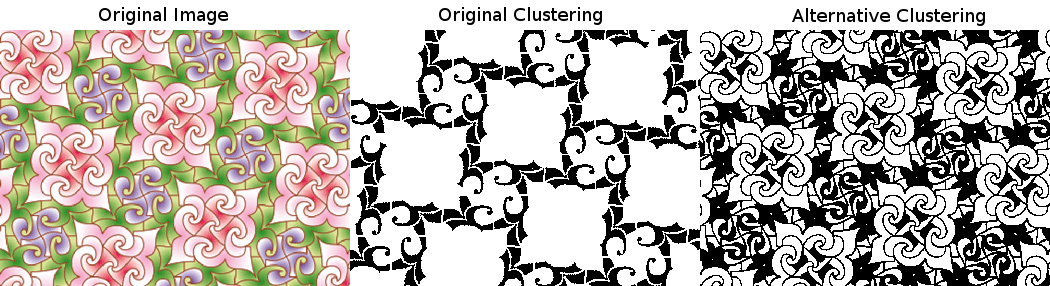
\includegraphics[scale=0.4]{./Figures/Etchers_result.png}
\caption{دسته‌بندی جایگزین برای یک پترن مخصوص}
\label{flowers}
\end{figure}

\subsubsection{بررسی زمان اجرا}
در این بخش، به بیان نتایج مقایسه‌ی الگوریتم 
\lr{ISM}
با سایر الگوریتم‌ها، از نظر زمان اجرا می‌پردازیم.

\begin{figure}[h!]
	\centering
	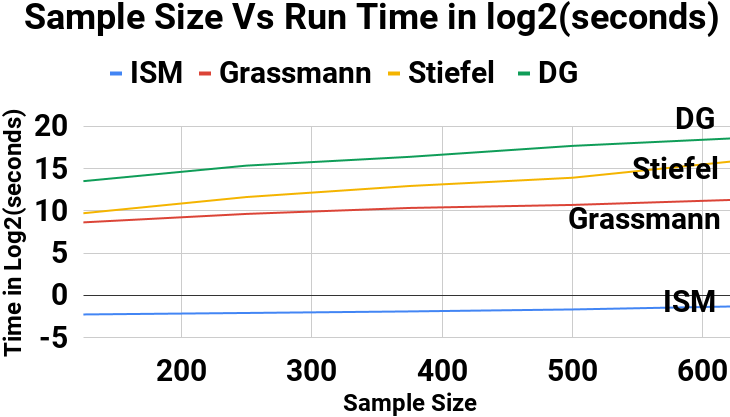
\includegraphics[scale = 0.35]{./Figures/runtime.png}
	\caption{زمان اجرای الگوریتم‌های مختلف بر جسب تعداد نمونه}
\end{figure}

مطابق انتظار، خم مربوط به الگوریتم 
\lr{ISM}
همواره پایین‌تر از منحنی سایر الگوریتم‌ها قرار دارد.
